\documentclass[dvipsnames]{acmart}

\usepackage{graphicx}
\usepackage{amssymb}
\usepackage{amsmath}
\usepackage{listings}
\usepackage{xcolor}
\usepackage{pgf,tikz}
\usepackage{multicol}
\usepackage{pgfplots}
\usetikzlibrary{positioning}

\title{Writing a CTLSKD Model-Checker in Ocaml}

\author{Aur\`ele Barri\`ere}

\date{December 2nd, 2018}

\lstset{language=[Objective]{Caml},
                basicstyle=\ttfamily\footnotesize,
                keywordstyle=\color{RedViolet}\ttfamily,
                stringstyle=\color{Violet}\ttfamily,
                commentstyle=\color{MidnightBlue}\ttfamily,
                morecomment=[l][\color{magenta}]{\#},
                morekeywords={bool, list, int},
                emph={%  
                  kripke, obs_marking, marking, state, std_state, std_kripke, std_marking, inf_set, observation, atp, ltl, state_ctls, path_ctls, history_ctlskd, path_ctlskd%
                },emphstyle={\color{Maroon}}
}

% macros
\def\ctls{CTL$^{*}$}
\def\ctlsk{CTL$^{*}$K}
\def\ctlskd{CTL$^{*}$K$\Delta$}
\def\ctlskdp{CTL$^{*}$K$\Delta\psi$}
\def\ltl{LTL}
\def\ap{AP}
\def\A{\mathit{A}}
\def\E{\mathit{E}}
\def\U{\mathit{U}}
\def\R{\mathit{R}}
\def\X{\mathit{X}}
\def\K{\mathit{K}}
\def\KP{\bar{\mathit{K}}}
\def\D#1{\Delta^{#1}}
\def\eq#1#2{\approx^{#2}_{#1}}
\def\eqh#1{\approx_{#1}}
\def\eqstate#1{\sim_{#1}}
\def\todo#1{{\color{red}#1}}
\def\iff{\ \mathit{iff}\ }
\def\UD{U_{\Delta}}
\def\UT{U_T}
\def\UDK#1{U_{\Delta #1}}
\def\UTK#1{U_{T #1}}
\def\FV{\mathit{FH}}
\def\FP{\mathit{FP}}
\def\ktree{$k$-tree}
\def\ktrees{$k$-trees}
\def\qed{\hfill$\blacksquare$}

\begin{document}
\maketitle

\section{Introduction}

Temporal Logics are a convenient formalism when it comes to reasoning about dynamic systems.
Similarly, Epistemic Logics allow to describe and reason about knowledge in distributed systems, or systems with imperfect information.
Combining the two kinds of logics for Epistemic Temporal Logics is a popular field with many uses, as in Artificial Intelligence or Game Theory.
In many real-world applications, several agents are involved, each with its own view of the world, and things evolve dynamically.

In an earlier work~\cite{internship}, we defined a new Epistemic Temporal Logic, \ctlskd.
It extends the \ctlsk\ logic, a well-known epistemic extension of \ctls, a popular temporal logic.
While \ctlsk\ added to \ctls\ the $\K$ operator to model agents knowledge, \ctlskd\ adds the operator $\Delta$, that allows agents to change their ``observational power'', or their point of view on the system.
For instance, the formula $\D{o}\K\A\X p$ means that after changing to an observation $o$, the agent knows that, on the next step, the proposition $p$ will hold, whatever path has been taken by the system.
To the best of our knowledge, this was the first time that such a change was enabled in an Epistemic Temporal Logic.

For Epistemic and/or Temporal Logics, model-checking (deciding if a formula is true in a model) is an important problem, as it allows to confront a specification and the modelization of a system.
In~\cite{internship}, we showed that model-checking \ctlskd\ could be reduced to the model-checking of \ctls. The model-checking of \ctls\ is itself known to be reducible to the model-checking of \ltl ~\cite{reduction}, another classical Temporal Logic.
We previously defined and model-checked \ctlskd\ in a multi-agent setting. However, this work will focus on the implementation of a single-agent \ctlskd\ model-checker. This choice was made for simplicity and the algorithm is almost identical.

In this report, I present my work on implementing a model-checker of \ctlskd. To this end, we use NuSMV~\cite{nusmv_paper}, a SAT-based \ltl\ model-checker, and build a \ctls\ model-checker, then a  \ctlskd\ model-checker, using the reductions.
The implementation is done in OCaml, and can be found online~\cite{ctlskd_mc}. In a first section, we present the logics and their formalization, then the reductions. We then discuss the implementation itself. Finally, we present a way to evaluate our implementation.


\section{Formally Model-Checking \ctlskd}
\label{formal}
Most of this section comes from our previous work~\cite{KR18,internship}. More details can be found there.
The following sections will only focus on new work.

\subsection{Single agent \ctlskd}
\subsubsection{Syntax}

We begin by introducing the syntax of \ctlskd. 
We consider $\mathcal{O}$ to be a set of \textit{observations}, that each represent a possible observational power of the agent. $\mathit{AP}$ is a set of atomic propositions.
Formulas of \ctlskd\ can be \textit{history formulas} $\varphi$ or \textit{path formulas} $\psi$.

$$\varphi := p ~|~ \neg \varphi ~|~ \varphi\wedge\varphi ~|~ \varphi\vee\varphi ~|~ \A\psi ~|~ \E\psi ~|~ \K\varphi ~|~ \D{o}\varphi$$
$$\psi := \varphi ~|~ \neg\psi ~|~ \psi\wedge\psi ~|~ \X\psi ~|~ \psi\U\psi$$

Where $p\in\mathit{AP}$ and $o\in\mathcal{O}$.
The temporal operators $\X$ and $\U$ are meant to represent the typical \textit{next} and \textit{until} operators of temporal logics.
$\A$ is a path quantifier, similar to those found in branching-time logics. Intuitively, $\A\psi$ should hold for a history if $\psi$ is true in every possible future. $\E$ is $\A$'s dual.
$\K$ is an epistemic operator. Intuitively, $\K\varphi$ should be true whenever the agent knows that $\varphi$ is true. We introduce a new one, $\D{o}$, to represent a change of observation.
$\varphi$ is called a history formula, as we only need to know what happened in the past to decide if the formula is true. $\psi$ is called a path formula as it also requires the future evolution of the system.

\paragraph{Models}
The models on which such formulas can be interpreted are classical Kripke Structure, with several equivalence relations between states (one for each observation). We note $M=(S,I_s,o_I,T,V,\eqstate{o_1},\dots,\eqstate{o_m})$.
A \textit{run} or \textit{path} is an infinite sequence of states $\pi=\pi_0\pi_1\dots$. A \textit{history} is a finite sequence of states $h=h_1\dots h_n$.


\subsubsection{Record Semantics}
We first define the natural semantics of \ctlskd. To this end, we first define Observation Records.

\paragraph{Observation records}
Given $\mathcal{O}$ a set of observations, we define \textit{observations records} to be ordered lists of pairs of observations and natural numbers.
Intuitively, an observation record represents changes of observations.

\textbf{Example:}  $r=[(o_1,0),(o_2,3),(o_3,3)]$ means that the player starts at time 0 with observation $o_1$. It keeps this observation, then at time 3, it first changes to $o_2$ and then to $o_3$. We use observation records in the semantics to remember the previous observations of the agent.

We write $r[(o,n)]$ to append a new pair $(o,n)$ to the observation record $r$.
We write $r_{\leq n}$ the record $r$ without the pairs $(o,m)$ where $m>n$.
We write $r_n$ the record $r$ without the pairs $(o,m)$ where $m\neq n$. 
We define a function $\mathit{O}(r,n)$ which gives a tuple of the observations used at time $n$. 

On a given model, with an observation record we can define an equivalence relation between histories, with regard to a record. Two histories are equivalent with regard to the record if the player can't distinguish them by using the observations in the record.\\
$h\eqh{r}h'\quad\iff\quad \forall i< |h|, \forall o\in \mathit{O}(r,i), h(i)\eqstate{o} h'(i)~\textit{and}~|h|=|h'|.$


Finally, the semantics are defined as follows:
History formulas need a history $h$ (finite sequence of previous states) and an observation record $r$ to be interpreted, to know which history might be considered possible for the agent.
Path formulas are interpreted on a run $\pi$ (infinite sequence of states of the model), a point in time (natural number), and an observation record.
\begin{table}
\begin{tabular}{l c l}
  $M,h,r \models p $&$ \iff $&$ p\in V(\mathit{last}(h))$\\
  $M,h,r \models \neg\varphi $&$ \iff $&$ M,h,r\not\models\varphi$\\
  $M,h,r \models \varphi_1\wedge\varphi_2 $&$ \iff $&$ (M,h,r\models\varphi_1~\text{and}~ M,h,r\models\varphi_2)$\\
  $M,h,r \models \varphi_1\vee\varphi_2 $&$ \iff $&$ (M,h,r\models\varphi_1~\text{or}~ M,h,r\models\varphi_2)$\\
  $M,h,r \models \A\psi  $&$ \iff $&$ \forall\pi$ that extends $h$, we have $M,\pi,|h|-1,r\models\psi$\\
  $M,h,r \models \E\psi  $&$ \iff $&$ \exists\pi$ that extends $h$, we have $M,\pi,|h|-1,r\models\psi$\\
  $M,h,r \models\K\varphi  $&$ \iff $&$ \forall h'$ such that $h'\eqh{r}h$, we have $M,h',r\models\varphi$\\
  $M,h,r \models \D{o}\varphi $&$ \iff $&$ M,h,r[(o,|h|-1)]\models\varphi$\\
  $M,\pi,n,r\models\varphi $&$ \iff $&$ M,(\pi_0\dots\pi_n),r\models\varphi$\\
  $M,\pi,n,r\models\neg\psi $&$ \iff $&$ M,\pi,n,r\not\models\psi$\\
  $M,\pi,n,r\models \psi_1\wedge\psi_2 $&$ \iff $&$ (M,\pi,r,n\models\psi_1~\text{and}~ M,\pi,r,n\models\psi_2)$\\
  $M,\pi,n,r\models\X\psi $&$ \iff $&$  M,\pi,(n+1),r\models\psi$\\
  $M,\pi,n,r\models \psi_1\U\psi_2 $&$ \iff $&$ \exists m\geq n$ such that $\forall k\in[n,m[, M,\pi,k,r\models\psi_1$ and $M,\pi,m,r\models\psi_2$\\
\end{tabular}
\end{table}

Finally, we say that $M=(S,I_s,o_I,T,V,\eqstate{o_1},\dots,\eqstate{o_m})$ models $\varphi$ (written $M\models\varphi$), if $\forall s\in I_s, M,s,[(o_I,0)]\models\varphi$. This definition corresponds to the model-checking problem.

\subsection{Model-Checking \ctlskd}
Because of perfect-recall semantics, it may seem that we have to remember the complete history and records when evaluating a formula. However, we can extract some information from the history that is sufficient for the evaluation of the formula. Intuitively, to evaluate a history formula, it is enough to know the current state, the current observation and the set of states that the agent believes the system might be in (called the \textit{Information Set}). This new structure to represent the knowledge is more succinct than remembering entire histories and records, as there is a finite number of information sets.

We define two functions to update information sets. $\UD$ updates the set when a player goes through a change of observation and $\UT$ updates the set when the player moves to a new state. 
\begin{tabular}{r c c c l}
$\UD(I,s,o)$& = &$\{x\in I$ & $|$ & $x\eqstate{o}s\}$\\
$\UT(I,s,o)$& = &$\{x\in S$ & $|$ & $\exists t\in I, t\rightarrow x ~\text{and}~ x\eqstate{o}s\}$\\
\end{tabular}

A few rules from this new semantics are:
\begin{tabular}{l c l}
  $M,s,I,o\models p $&$ \iff $&$ p\in V(s)$\\
  $M,s,I,o\models\A\psi $&$ \iff $&$ \forall\pi$ such that $\pi_0=s$, we have $M,\pi,I,o\models\psi$\\
  $M,s,I,o\models\K\varphi $&$ \iff $&$ \forall s'\in I$, we have $M,s',I,o\models\varphi$\\
  $M,s,I,o'\models\D{o}\varphi $&$ \iff $&$ M,s,\UD(I,s,o),o\models\varphi$\\
  $M,\pi,I,o\models\X\psi $&$ \iff $&$ M,\pi_{1\dots},\UT(I,\pi_1,o),o\models\psi$\\
\end{tabular}

We proved in~\cite{internship} the following theorem:
$\forall \varphi,h,r,s,I,o$ such that $\FV(h,r)=(s,I,o)$, $M,h,r\models\varphi\iff M,s,I,o\models\varphi$.
Where $\FV$ is a function that relates histories and observation records to the corresponding current state, information set and observation.
This proves that the two semantics are equivalent, and it suffices to model-check the information set semantics.

To this end, from $M=(S,I,o_I,T,V,\eqstate{o_1},\dots,\eqstate{o_m})$ we define the augmented model $\hat{M}=(S',T',V')$, a Kripke Structure.
\begin{itemize}
\item $S'=S\times 2^{S}\times \mathcal{O}$: states are state of the original model, an observation set and an observation.
\item $(s,I,o)~T'~(s',I',o)\iff s~T~s'$ and $I'=\UT(I,s',o)$
\item $V'(s,I,o)=V(s)$. As the algorithm is executed, new atomic propositions will appear.
\end{itemize}

Finally, any formula of \ctlskd\ can be model-checked with a marking algorithm on the (finite) augmented model.
Intuitively, for each $\D{o}\varphi$ where $\varphi$ is a \ctls\ formula, we model-check $\varphi$ on each state of $\hat{M}$.
Then, we mark each state $(s,I,o')$ of $\hat{M}$ with a new atomic proposition if $\varphi$ holds on $(s,\UD(I,s,o),o)$.
Similarly for formulas $\K\varphi$ where $\varphi$ is a \ctls\ formula, a state $(s,I,o)$ is marked with a new atomic proposition if $\varphi$ holds in each $(s',I,o)$ where $s'\in I$.

Finally, we replace either $\D{o}\varphi$ or $\K\varphi$ in the formula with the new atomic proposition, and start from the beginning until there are no more $\K$ or $\Delta$ operators in the formula. The remaining formula can be model-checked with the \ctls\ model-checker.

The definition of the Information Set semantics makes the correctness of the algorithm almost trivial.

\section{Our Approach to Implementing a \ctlskd\ model-checker}

\subsection{Types}
Our models can either be standard models, where each state can be numbered, or augmented models for the model-checking of \ctlskd.
States of augmented models include a standard state, an information set and an observation

We thus define our states as such:
\begin{lstlisting}
  type std_state = int
  type inf_set = std_state list
  type state = I of std_state
             | A of std_state * inf_set * observation
\end{lstlisting}

When building augmented states, we make sure that the information sets have no duplicates and are ordered, which guarantees that each augmented state has a unique representation.

Kripke structures are then defined. The \lstinline{kripke} type represents the states and transition of a Kripke Structure: each element of the list is a state and its list of successors.
A marking represents the valuation function. Each element of the list contains an atomic proposition and the list of states where it holds.
Decoupling the two types allows to add new atomic propositions without changing the underlying structure, which will prove useful for marking algorithms.
Observations equivalence relations are described with the \lstinline{obs_marking} type. It maps observations and states to a value. 

\begin{lstlisting}
  type kripke = (state * state list) list
  type std_kripke = (std_state * std_state list) list
  type marking = (atp * state list) list
  type std_marking = (atp * std_state list) list
  module ObsMap = Map.Make(struct type t = (observation * std_state) let compare = compare end)
  type obs_marking = int ObsMap.t
  let eq_state (om:obs_marking) (o:observation) (s1:std_state) (s2:std_state): bool =
    ObsMap.find (o,s1) om = ObsMap.find (o,s2) om
\end{lstlisting}


We then define the 3 logics' syntaxes:
\begin{center}
  \begin{minipage}[t]{0.4\linewidth}
\begin{lstlisting}
type ltl =
  | LTL_TRUE
  | LTL_AP of atp
  | LTL_NEG of ltl
  | LTL_OR of ltl * ltl
  | LTL_AND of ltl * ltl
  | LTL_X of ltl
  | LTL_U of ltl * ltl

type state_ctls =
  | ST_CTLS_TRUE
  | ST_CTLS_AP of atp
  | ST_CTLS_NEG of state_ctls
  | ST_CTLS_OR of state_ctls * state_ctls
  | ST_CTLS_AND of state_ctls * state_ctls
  | ST_CTLS_A of path_ctls
  | ST_CTLS_E of path_ctls
 and path_ctls =
   | P_CTLS_S of state_ctls
   | P_CTLS_NEG of path_ctls
   | P_CTLS_OR of path_ctls * path_ctls
   | P_CTLS_AND of path_ctls * path_ctls
   | P_CTLS_X of path_ctls
   | P_CTLS_U of path_ctls * path_ctls
 \end{lstlisting}
\end{minipage}
\begin{minipage}[t]{0.5\linewidth}
\begin{lstlisting}
type history_ctlskd =
  | H_CTLSKD_TRUE
  | H_CTLSKD_AP of atp
  | H_CTLSKD_NEG of history_ctlskd
  | H_CTLSKD_OR of history_ctlskd * history_ctlskd
  | H_CTLSKD_AND of history_ctlskd * history_ctlskd
  | H_CTLSKD_A of path_ctlskd
  | H_CTLSKD_E of path_ctlskd
  | H_CTLSKD_K of history_ctlskd
  | H_CTLSKD_D of observation * history_ctlskd
 and path_ctlskd =
   | P_CTLSKD_H of history_ctlskd
   | P_CTLSKD_NEG of path_ctlskd
   | P_CTLSKD_OR of path_ctlskd * path_ctlskd
   | P_CTLSKD_AND of path_ctlskd * path_ctlskd
   | P_CTLSKD_X of path_ctlskd
   | P_CTLSKD_U of path_ctlskd * path_ctlskd
\end{lstlisting}
\end{minipage}
\end{center}

Given these types, we can define the signature of our 3 model-checking procedures:

\begin{lstlisting}
  let ltl_mc (k:kripke) (init:state) (m:marking) (spec:ltl): bool = ...
  let ctls_mc (k:kripke) (init:state) (m:marking) (spec:state_ctls): bool = ...
  let ctlskd_mc (k:std_kripke) (state_init:std_state) (m:std_marking) (obs_init:observation)
                (om:obs_marking) (spec:history_ctlskd): bool = ...
\end{lstlisting}

Notice how \ltl\ and \ctls\ model-checkers take as input generic kripke structure (either standard or augmented), while the \ctlskd\ function takes a standard kripke structure. It will then build the augmented model and give it to the \ctls\ function, which in turn calls the \ltl\ one on the same model.
Similarly, as only \ctlskd\ has imperfect information, its function is the only one requiring an observation marking and an initial observation.

\subsection{\ltl\ Model-Checking}
As we use NuSMV, a \ltl\ and CTL model-checker, our model-checking procedure can simply call it.
However, NuSMV only works on an input file. We then write several functions to translate a \ltl\ model-checking problem as a file following the syntax of NuSMV.
We then call the NuSMV executable on this file. Because its output is a long string, we write a small wrapper in C to analyze it and simply return 1 or 0 depending on the result. This returned value can be obtained in Ocaml by using the \lstinline{Sys.command} function.

\subsection{\ctls\ Model-Checking}
An algorithm to create a \ctls\ model-checker from a \ltl\ one can be seen in~\cite{reduction}.
This is a simple marking algorithm on formulas of the form $\E\varphi$.

However, in this algorithm, the authors assume that the \ltl\ model-checking procedure returns true if the formula is true in at least one path starting from the initial state (\ltl\ formulas are evaluated on paths).
NuSMV returns true if the formula holds in all paths starting from the initial state.
We thus adapt the algorithm to mark on all sub-formulas $\A\varphi$, and replace each $\E\varphi$ with $\neg\A\neg\varphi$.

Finally, all the marking algorithms from~\cite{reduction} and~\cite{internship} were written in an imperative way.
We design a marking recursive function for functional languages.
We use the pattern-matching feature of OCaml to match on the inductive structure of formulas to model-check.
In practice, our function has the following signature:

\begin{lstlisting}
  let rec marking_update (k:kripke) (m:marking) (spec:state_ctls): (marking * state_ctls) = ...
  and path_marking_update (k:kripke) (m:marking) (spec:path_ctls): (marking * path_ctls) = ...
\end{lstlisting}

This function takes a structure (with its marking of atomic propositions) and a specification. It returns a new marking and a new specification, where in the new formula, each sub-formula $\A\varphi$ has been replaced with a fresh atomic proposition, and the new marking contains the truth assignment for each of these new propositions.

Most cases simply call the function recursively on subformulas:
\begin{lstlisting}
    | ST_CTLS_OR (s1,s2) -> let (newm1, newspec1) = marking_update k m s1 in
                          let (newm2, newspec2) = marking_update k newm1 s2 in
                          (newm2, ST_CTLS_OR (newspec1, newspec2))
\end{lstlisting}

When dealing with an $\A\varphi$, we call the model-checker on each states to mark the correct states (function \lstinline{check_ltl} calls \lstinline{ltl_mc} on all states), and replace $\A\varphi$ with the proposition \lstinline{fresh}:
\begin{lstlisting}
  | ST_CTLS_A p ->
     begin match is_linear_ctls p with
     | true -> let fresh = fresh_atp m in
               let newm = (fresh, check_ltl k m (linear_ctls_to_ltl p))::m in
               (newm, ST_CTLS_AP fresh)
     | false -> let (newm, newspec) = path_marking_update k m p in
                marking_update k newm (ST_CTLS_A newspec)
     end
\end{lstlisting}
Note that, if $\varphi$ is not a linear formula, we don't replace it right away, as the \ltl\ procedure only deals with \ltl\ formulas. In that case, we first replace the inner sub-formulas.

We have one such case for each possible inductive case. We don't define any for $\E\varphi$ as we replaced them earlier.
Finally, the \lstinline{marking_update} function returns a new marking and a new specification. This formula is linear (no more $\A\varphi$), and checking it in \ltl\ with the new marking is equivalent to model-checking the original problem.

\subsection{\ctlskd\ Model-Checking}
As seen on section~\ref{formal}, model-checking \ctlskd\ can be done once again with a marking algorithm.
However, this marking operates on the augmented model.
We first define functions to build an augmented model (along with its valuation of atomic propositions) from a standard kripke structure.

\begin{lstlisting}
  let augmented_kripke (k:std_kripke) (obs:observation list) (om:obs_marking): kripke = ...
  let rec augmented_marking (m:std_marking) (states: state list): marking = ...
\end{lstlisting}

We can then define the marking algorithm in a similar way as \ctls. This time, the formulas that will be replaced by fresh atomic propositions are $\K\varphi$ and $\D{o}\varphi$, where $\varphi$ is a \ctls\ formula. More details can be found in~\cite{internship}.
For instance, for $\D{o}\varphi$ formulas:
\begin{lstlisting}
  | H_CTLSKD_D (o,h) ->
     begin match (is_history_ctls h) with
     | true -> let states_h_true = check_ctls k m (history_ctlskd_to_ctls h) in
               let fresh = fresh_atp m in
               let newm = (fresh, List.filter (filter_delta om states_h_true o) (get_states k))::m in
               (newm, H_CTLSKD_AP fresh)
     | false -> let (newm, newspec) = aug_marking_update k m om h in
                aug_marking_update k newm om (H_CTLSKD_D (o,newspec))
     end
\end{lstlisting}


\section{Evaluation}
Our implementation was successfully written in Ocaml. It is available online~\cite{ctlskd_mc}, but requires a NuSMV executable (also available online for free~\cite{get_nusmv}). It required over 800 lines of commented OCaml and a small NuSMV wrapper written in C.

Only the model-checking procedures were implemented, meaning that there is currently no parser to get a formula and a model. One has to write directly in the Ocaml syntax, which makes for unnecessary long definitions.

To evaluate our implementation, we first wrote a few generic tests on small models, such that we could know the answer.
All of these tests return the expected result.

We then created parametric tests for each of our logics. These take 2 arguments (the model's size and the formula's size), build a problem and solve it. This allows to study the time complexity of our procedures. We picked these models and formulas for their simplicity and our ability to predict their results (to check for any errors in the implementation).

\begin{figure}[!tbp!h]
  \centering
  \begin{minipage}[b]{0.4\textwidth}
    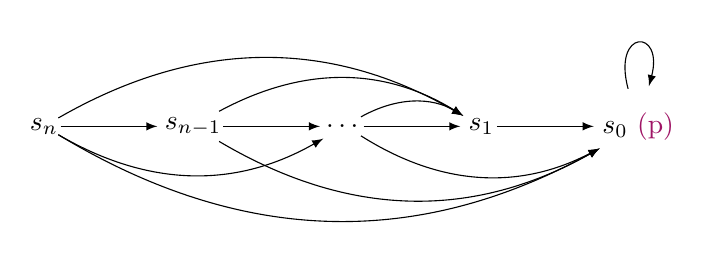
\begin{tikzpicture}[%
        every node/.style={circle,minimum size=4pt,minimum height=4pt, inner sep=0pt},
        shorten >=2pt,
        node distance=1.3cm, >=latex
      ]
      \node [] (0) [circle] {$s_n$};
      \node [] (1) [circle, right=of 0] {$s_{n-1}$};
      \node [] (2) [circle, right=of 1] {$\dots$};
      \node [] (3) [circle, right=of 2] {$s_1$};
      \node [] (4) [circle, right=of 3] {$s_0$~\color{RedViolet}(p)};
      \path [draw] (0) edge[->]  node {} (1)
      (1) edge[->]  node {} (2)
      (2) edge[->]  node {} (3)
      (3) edge[->]  node {} (4)
      (2) edge[->, bend right]  node {} (4)
      (1) edge[->, bend right]  node {} (4)
      (0) edge[->, bend right]  node {} (4)
      (2) edge[->, bend left]  node {} (3)
      (1) edge[->, bend left]  node {} (3)
      (0) edge[->, bend left]  node {} (3)
      (0) edge[->, bend right]  node {} (2)
      (4) edge[->,loop above]  node {} (4);
    \end{tikzpicture}
    \caption{Parametric Model for \ltl}
    \label{model_ltl}
  \end{minipage}
  \hfill
  \begin{minipage}[b]{0.4\textwidth}
    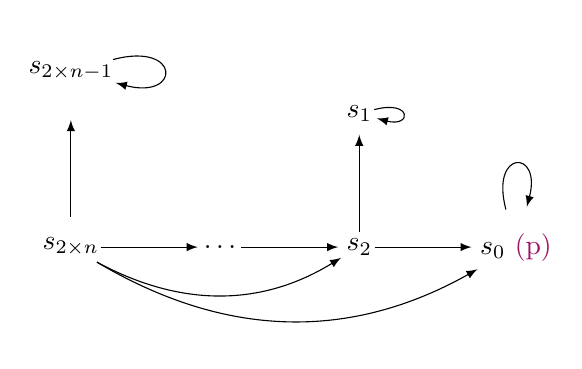
\begin{tikzpicture}[%
        every node/.style={circle,minimum size=4pt,minimum height=4pt, inner sep=0pt},
        shorten >=2pt,
        node distance=1.3cm, >=latex
      ]
      \node [] (0) [circle] {$s_{2\times n}$};
      \node [] (1) [circle, above=of 0] {$s_{2\times n-1}$};
      \node [] (2) [circle, right=of 0] {$\dots$};
      \node [] (3) [circle, right=of 2] {$s_2$};
      \node [] (4) [circle, above=of 3] {$s_1$};
      \node [] (5) [circle, right=of 3] {$s_0$~\color{RedViolet}(p)};
      \path [draw] (0) edge[->]  node {} (1)
      (3) edge[->]  node {} (4)
      (3) edge[->]  node {} (5)
      (2) edge[->]  node {} (3)
      (0) edge[->]  node {} (2)
      (0) edge[->, bend right]  node {} (3)
      (0) edge[->, bend right]  node {} (5)
      (1) edge[->, loop right]  node {} (1)
      (4) edge[->, loop right]  node {} (4)
      (5) edge[->, loop above]  node {} (5);
    \end{tikzpicture}
    \caption{Parametric Model for \ctls}
  \label{model_ctls}
  \end{minipage}
\end{figure}

\begin{figure}[!h]
  \centering
  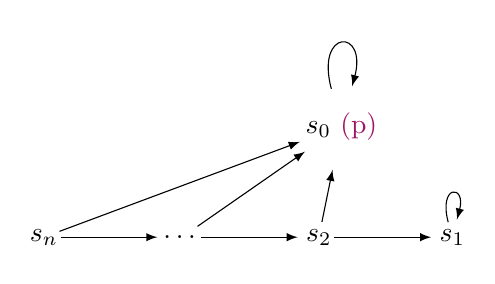
\begin{tikzpicture}[%
      every node/.style={circle,minimum size=4pt,minimum height=4pt, inner sep=0pt},
      shorten >=2pt,
      node distance=1.3cm, >=latex
    ]
    \node [] (0) [circle] {$s_0$~\color{RedViolet}(p)};
    \node [] (1) [circle, below right=of 0] {$s_1$};
    \node [] (2) [circle, left=of 1] {$s_2$};
    \node [] (3) [circle, left=of 2] {$\dots$};
    \node [] (4) [circle, left=of 3] {$s_n$};
    \path [draw] (2) edge[->]  node {} (1)
    (3) edge[->]  node {} (2)
    (4) edge[->]  node {} (3)
    (2) edge[->]  node {} (0)
    (3) edge[->]  node {} (0)
    (4) edge[->]  node {} (0)
    (0) edge[->, loop above]  node {} (0)
    (1) edge[->, loop above]  node {} (1);
  \end{tikzpicture}
  \caption{Parametric Model for \ctlskd}
  \label{model_ctlskd}
\end{figure}

\subsection{Evaluation Setting}
\paragraph{Evaluating \ltl}
Given a size $n$, we build the model that can be seen on Figure~\ref{model_ltl}.
Given a formula size $m$, we build the following specification:
$\phi_0 = (true~\U~p)$,\quad $\phi_{m+1} = true~\U~\X (\phi_m)$.
We can easily check that, for any formula size and model size, the formula holds (with initial state $s_n$).

The Figure~\ref{time_ltl} gives the time it took for our solver to build the example and find that result, for different values of $m$ and $n$.

\paragraph{Evaluating \ctls}
The parametric model is given Figure~\ref{model_ctls}.
The formulas are $\phi_0 = \E(true~\U~p)$\quad$\phi_{m+1} = \E\X\phi_m$.
The Figure~\ref{time_ctls} gives the results.

\paragraph{Evaluating \ctlskd}
The parametric model is given Figure~\ref{model_ctlskd}.
The formulas are $\phi_0 = \D{o_2}\K\neg p$\quad$\phi_{m+1} =\E\X\phi_m$.
The Figure~\ref{time_ctls} gives the results.
The initial observation is $o_1$, the blind observation where all states are indistinguishables.
The observation $o_2$ is the perfect one, where the agent can distinguish each state.
The initial state is $s_n$.

\subsection{Result analysis}
As we only checked our procedures on one example each, the depicted results are not enough to make general assumptions about the performance and complexity of our algorithms, but they provide a valuable insight.
First, we know that both \ltl\ and \ctls\ model-checking problems are in PSPACE-complete~\cite{complexity}. We showed in~\cite{KR18} that the single-agent \ctlskd\ model-checking problem is in EXPTIME. However, no lower-bounds have been established yet.

We can see that both marking algorithm (for \ctls\ and \ctlskd) seem to behave linearly in the size of the formula.
Indeed, in our examples, the constructors are all nested.
Consider the formulas $\phi_0 = \E(true~\U~p)$\quad$\phi_{m+1} = \E\X\phi_m$.
When model-checking $\phi_m$ on a model, we first model-check $\phi_0$ on each states of the augmented model, and add a new marking.
We then model-check the formula $\E\X a$, where $a$ is a new atomic proposition (true on the states where $\phi_0$ holds).
In general, to model-check $\phi_{m+1}$, we model-check the formula $\E\X q$ where q is an atomic proposition true on states where $\phi_m$ holds.
This amounts to using NuSMV on the \ltl\ formula $\neg\X q$.
The time to model-check this formula does not depend on $m$, as the entire formula $\phi_m$ has been reduced to a simple atomic proposition.
This explains why our marking algorithms are linear in the size of the formulas in our examples.

Finally, the number of states in the augmented model is easily computable: $|S|\times 2^{|S|-1}\times |\mathcal{O}|$ (we only build the states $(s,I,o)$ where $s\in I$, as the others are not reachable). This explains why the time of model-checking \ctlskd\ explodes so quickly in Figure~\ref{time_ctlskd}.

\newcommand\plotscale{0.8}
\begin{figure}
  \begin{tikzpicture}[scale=\plotscale]
    \begin{axis}[ xlabel=Model size (with formula size 10), ylabel=Time (seconds)]
      \addplot[color=RedViolet,mark=x] coordinates {
        (10,0.018)
        (50,0.037)
        (100,0.019)
        (150,0.295)
        (200,0.607)
        (250,1.104)
        (300,1.778)
        (350,3.095)
        (400,4.150)
        (450,5.903)
        (500,9.217) };
    \end{axis}
  \end{tikzpicture}%
  \begin{tikzpicture}[scale=\plotscale]
    \begin{axis}[ xlabel=Formula size (with model size 20), ylabel=Time (seconds)]
      \addplot[color=RedViolet,mark=x] coordinates {
        (10,0.019)
        (50,0.05)
        (100,0.150)
        (150,0.470)
        (200,1.046)
        (250,1.857)
        (300,3.628)
        (350,5.556)
        (400,7.942)
        (450,12.762)
        (500,16.9) };
    \end{axis}
  \end{tikzpicture}
  \caption{LTL Time Results}
  \label{time_ltl}
\end{figure}

\begin{figure}
  \begin{tikzpicture}[scale=\plotscale]
    \begin{axis}[ xlabel=Model size (with formula size 5), ylabel=Time (seconds)]
      \addplot[color=RedViolet,mark=x] coordinates {
        (1,0.206)
        (5,0.788)
        (10,1.685)
        (15,2.815)
        (20,4.370)
        (25,6.464)
        (30,9.09)
        (35,12.709)
        (40,16.969)
        (45,22.424)
        (50,29.349) };
    \end{axis}
  \end{tikzpicture}%
  \begin{tikzpicture}[scale=\plotscale]
    \begin{axis}[ xlabel=Formula size (with model size 5), ylabel=Time (seconds)]
      \addplot[color=RedViolet,mark=x] coordinates {
        (1,0.267)
        (10,1.432)
        (20,2.763)
        (30,4.210)
        (40,5.709)
        (50,7.236)
        (60,8.905)
        (70,10.501)
        (80,12.240)
        (90,14.158)
        (100,16.060) };
    \end{axis}
  \end{tikzpicture}
  \caption{\ctls\ Time Results}
  \label{time_ctls}
\end{figure}

\begin{figure}
  \begin{tikzpicture}[scale=\plotscale]
    \begin{axis}[ xlabel=Model size (with formula size 1), ylabel=Time (seconds)]
      \addplot[color=RedViolet,mark=x] coordinates {
        (1,0.251)
        (2,0.844)
        (3,3.094)
        (4,15.867)
        (5,116.823) };
    \end{axis}
  \end{tikzpicture}%
  \begin{tikzpicture}[scale=\plotscale]
    \begin{axis}[ xlabel=Formula size (with model size 2), ylabel=Time (seconds)]
      \addplot[color=RedViolet,mark=x] coordinates {
        (1,0.843)
        (2,1.161)
        (3,1.461)
        (4,1.770)
        (5,2.099)
        (6,2.420)
        (7,2.742)
        (8,3.064)
        (9,3.390)
        (10,3.703) };
    \end{axis}
  \end{tikzpicture}
  \caption{\ctlskd\ Time Results}
  \label{time_ctlskd}
\end{figure}

\section{Future Works}
Our implementation seems to give correct results so far, but could be improved in numerous ways.

\paragraph{Parsing}
We could allow the user to write an input file in a given syntax (maybe the same as NuSMV's).

\paragraph{Multi-Agent}
In~\cite{KR18}, we define \ctlskd\ for multi agent settings. Each $\K$ and $\Delta$ operators takes an additional parameter to indicate the relevant agent.
We showed that the model-checking algorithm is almost identical, but needs to use $k$-trees instead of Information Sets (a tree that represents one agent's knowledge of the other agents' knowledge, introduced in~\cite{ktrees}).
This would be an easy extension to our implementation.

\paragraph{Polymorphism}
We didn't use all the polymorphic features of OCaml. A more elegant way to define models would have been to use a more abstract type for states. We kept it simple for this proof-of-concept implementation.

\paragraph{Other Solvers}
We currently only use NuSMV, but there are numerous other \ltl\ solvers. Another good choice would have been SPIN~\cite{spin}.
It would be interesting to compare the results in our setting.

\paragraph{Binding NuSMV}
In this version, we write to a file each \ltl\ problem for NuSMV to parse and solve. We might be losing a lot of time doing useless writing and parsing (our representation is already parsed). A good solution would be to bind our representation to NuSMV's, and call their own functions directly. Such C-OCaml interfacing can be done, but would require some time to understand NuSMV's code.

\paragraph{Data structures}
As the augmented model grows exponentially in the size of the original model, keeping a list of states and transitions might not be the most optimal choice.

\paragraph{Splitting the augmented model}
In our \ctlskd\ model-checking procedure, we give the entire augmented model to the \ctls\ model-checker.
However, the augmented model is actually composed of $o$ disjoint components, where $o$ is the number of observations.
As \ctls\ and \ltl\ model-checking complexity depends on the size of the model, we could probably save some time by giving them the appropriate component of the augmented model. If NuSMV performs reachable state analysis, this would only save the time of writing and parsing too many states and transitions.

\paragraph{Counter-Example generation}
NuSMV finds a counter-example in false specifications. We believe that, using these counter-examples, we could build one for the \ctlskd\ model-checking problem. However, NuSMV's output when printing a counter-example isn't directly exploitable (states are renamed for instance). 

\section{Acknowledgments}
I am grateful to Bastien Maubert, Sasha Rubin and Aniello Murano for working with me on \cite{internship,KR18}, and advising me on this project.
In particular, they redirected me to NuSMV and SPIN, and towards the reduction from \ctls\ to \ltl\ in~\cite{reduction}.

\section{Related Works and Conclusion}
Our previous work already defined \ctlskd. Our implementation is based on the model-checking procedure we wrote in~\cite{internship}.
The reduction technique resembles other algorithms from model-checking.
Marking algorithms have been used previously (in~\cite{reduction} for instance).
However, all implementations in the literature seem to be written in an imperative way.
Information Sets are a particular case of $k$-trees~\cite{ktrees}.

We implemented a \ctlskd\ model-checker in OCaml. We make use of its functional features to implement functional marking algorithms. The model-checking problem was solved in~\cite{internship} by means of a reduction to \ctls\ model-checking. 

The functional style of OCaml makes for elegant definitions of logics and marking algorithms. However, we still have a long way to go before this can check large models in a reasonable time. Part of it comes from the complexity of \ctlskd\ model-checking in itself, but we could also optimize our implementation.
Nevertheless, our implementation has given a correct results on all of our tests.

\newpage
\bibliographystyle{plain}
\bibliography{report}

\end{document}
